\documentclass{exam}

\usepackage[margin=1in]{geometry}

\usepackage{comment}
\usepackage{graphicx}
\usepackage{listings}

\pagestyle{headandfoot}
\firstpageheader{CSCI 389}{}{Processor Architecture Assignment}
\runningheader{CSCI 389}{}{Processor Architecture Assignment}


\begin{document}
\title{Processor Architecture Assignment (Learning)}
\author{CSCI 389: Computer Systems}
\date{Fall 2021}
\maketitle


This assignment is an opportunity to test your understanding of processor architecture and receive feedback. 
Point values are assigned so that you can differentiate between large and small mistakes, but this assignment does not affect your grade. 

\textbf{Due Date:}
Friday, February 11th at 10:00 am. 

\begin{questions}

\question[8]
\textbf{Decoding Assembly.}
Using the ALPHA instruction set (from the Processor Architecture Slides), decode the following hexadecimal instructions. 
This is a four step process: 
1. Convert the instruction to binary. 
2. Map the binary bits to the different fields of the instruction (use the opcode to determine instruction type). 
3. Convert the values of the different fields of the instruction from binary to hexadecimal. 
4. Check the opcode (and perhaps func field) for the type of operation and the arguments. 
Specify the operation type. The arguments can be left in hexadecimal, but specify input vs output. 
\begin{parts}
\part[4]
0x44720805
\part[4]
0xb532bad4
\end{parts}

\textbf{A.}

Binary is: $0100 0100 0111 0010 0000 1000 0000 0101$

Opfield = $0100 01_{2}=11_{16}$

RA = $00 011_{2}= 3$

twelth bit = 0

RB = $1 0010_{2}=12_{16}$

Funct = $1000 000_{2}=40$ (XOR)

RC = $0 0101_{2}=05$

Translated XOR R3 with R12 place in R5. 

\textbf{B.}

Binary is $1011 0101 0011 0010 1011 1010 1101 0100$

Opfield is $1011 01_{2}=2D_{16}$

RA is $01 001_{2}=19_{16}$

RB = $1 0010_{2}=14_{12}$

Offset is: $1011 1010 1101 0100_{2}=BAD4_{16}$

Translated is Store R19 in R19 offset by $BAD4$

\question[12]
\textbf{Latency and Bandwidth.}
Consider the pipeline architectures shown below:
\begin{center}
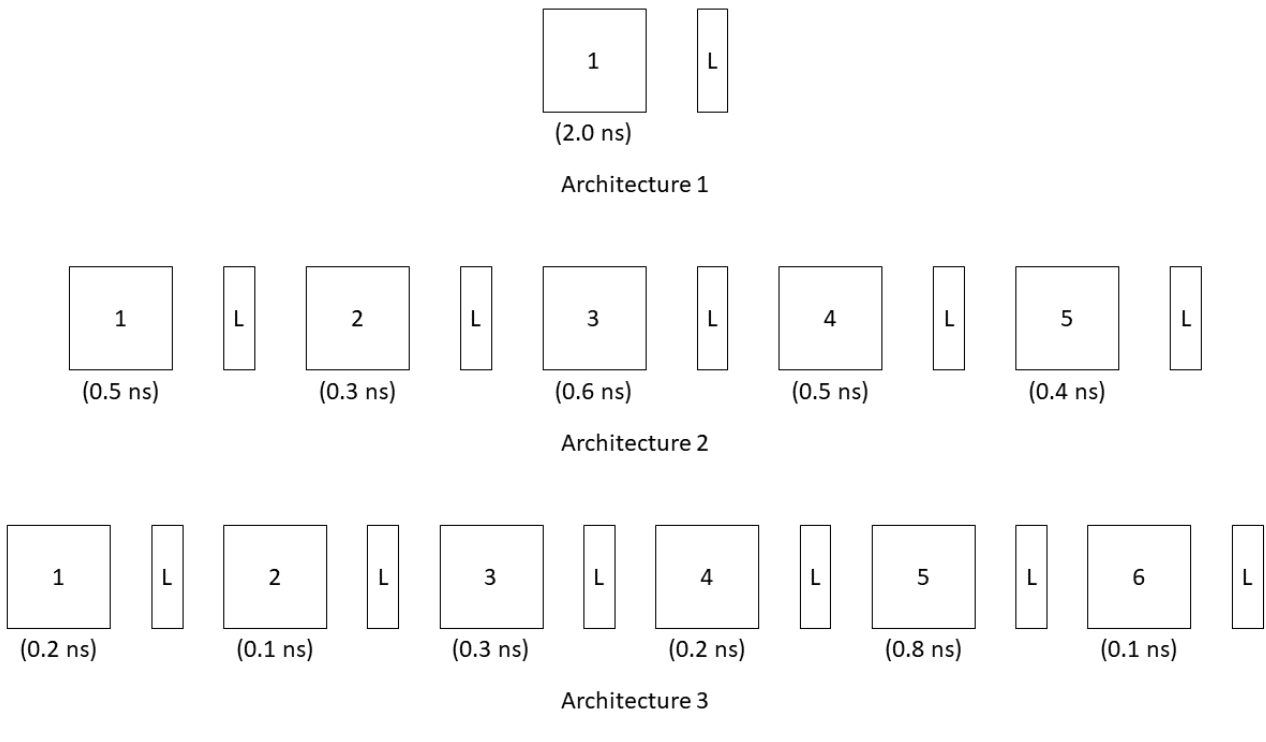
\includegraphics[width=0.6\textwidth{}]{architecture.png}
\end{center}
Compute the latency and bandwidth for each architecture, assuming that latches (registers) take 0.1 ns. 

\begin{parts}
\part[4]
Architecture 1. 

\part[4]
Architecture 2. 

\part[4]
Architecture 3. 

\end{parts}

$\mathrm{latency}=\mathrm{num\ stages} \cdot (\mathrm{max\ stage\ time})$

$\mathrm{bandwidth} = \frac{1}{\mathrm{Max\ stage\ time}}$


\textbf{A.} $\mathrm{Latency}=1 \cdot (2+0.1)=2.1$ ns

$\mathrm{bandwidth} = \frac{1}{\mathrm{2.1}}=0..47$ Ghz


\textbf{B.} $\mathrm{Latency}= 5\cdot (0.6+0.1)=5 \cdot 0.7 = 3.5$ ns

$\mathrm{bandwidth} = \frac{1}{\mathrm{0.7}}= 1.43$ Ghz


\textbf{C.} $\mathrm{Latency}= 6\cdot (0.8+0.1)=6 \cdot 0.9 = 5.4$ ns

$\mathrm{bandwidth} = \frac{1}{\mathrm{0.9}}=1.\overline{11}$ Ghz


\question[20]
\textbf{Analyzing Code Execution.}
Consider the following instructions:
\begin{lstlisting}
00 loop:
01 r1 * 8 => r4
02 r2 + r4 => r5
03 r3 + r4 => r6
04 load[r5 + 0] => r7
05 load[r6 + 0] => r8
06 r7 * r8 => r5
07 r1 * 2 => r6
08 r5 + r6 => r5
09 store r5 => [r4 + 0]
10 r1 + 1 => r1
11 compare r1, r10
12 branch if not zero => loop
\end{lstlisting}
\begin{parts}
\part[4]
List the data hazards for the instruction 04. For each hazard, label its type. 

\part[4]
List the data hazards for the instruction 09. For each hazard, label its type. 

\part[12]
Draw a pipeline diagram showing the progression of one iteration of these instructions through a basic 5-stage pipeline that has EX-EX, MEM-MEM, and MEM-EX forwarding, but lacks more advanced parallelism techniques. 
Make sure to label all instances of forwarding. 
\end{parts}


\textbf{A.}

RAW hazard from line 2

\textbf{B.}

RAW hazard. R5 is written on line 8 but can be prempticely read on line 9


WAW R4 can be clobbered on line 1



\question[5]
\textbf{Loop Unrolling.}
Consider the following instructions:
\begin{lstlisting}
loop:
load[r1 + 0] => r3
r2 + r3 => r2
store r2 => [r1 + 0]
r1 + 8 => r1
branch if r1 < r4 => loop
\end{lstlisting}
Unroll this loop so that 4 iterations happen between branches. 
Make sure that your unrolled loop is correct. 
%Don't worry about the edge case of fewer than 4 iterations. 

\begin{lstlisting}
loop:
load[r1 + 0] => r3
r2 + r3 => r2
store r2 => [r1 + 0]
r1 + 8 => r1
load[r1 + 0] => r3
r2 + r3 => r2
store r2 => [r1 + 0]
r1 + 8 => r1
branch if r1+1 < r4 => loop

load[r1 + 0] => r3
r2 + r3 => r2
store r2 => [r1 + 0]
r1 + 8 => r1
\end{lstlisting}

\end{questions}

\end{document}